\documentclass{aa}
\usepackage[varg]{txfonts}
\usepackage{nicefrac}
\usepackage{caption}
\usepackage{listings}
\usepackage{color}

\definecolor{paper}{RGB}{235,213,179}
\definecolor{orange}{RGB}{255,79,0}

\begin{document}

\lstset{language=Python,
        xleftmargin=2em,
        backgroundcolor=\color{paper},
        numbers=left,
        numbersep=5pt,
        numberstyle=\tiny,
        rulecolor=\color{black},
        keywordstyle=\color{orange},
        basicstyle=\footnotesize,
        breaklines=true,
        breakatwhitespace=true}

\title{Assignment 2}

\subtitle{Numerical Ordinary Differential Equation solvers.}

\author{David Hernandez\inst{1}}


\institute{Universität Wien, Institut für Astrophysik, Türkenschanzstrasse
17, 1180 Wien, Austria}

\date{Deadline: November 30\textsuperscript{th}, 2020 / Submitted: }

\abstract{In astronomy it is often necessary to solve differential equations for which no
analytic solutions exist, or are extremely hard to compute. Another aspect that can stand in
the way of solving the problem by hand is a large number of individual computations, as is the
case with N-Body simulations. Therefor, numerical ODE-Solvers can be immensely useful. We shall
implement five different methods and analyze their performance and compare the results. This
work is divided into two parts. In the first part four approaches (Forward Euler, Classical
Runge-Kutta, Backward Euler and Crank-Nicolson) with a fixed time step length
\(\Delta t\) are implemented, whereas the in the second part we shall take a closer look at a
method with variable time step length (Runge-Kutta-Fehlberg).}

\keywords{Numerical methods -- ODE-Solvers -- Forward-Euler -- Backward-Euler
-- Crank-Nicolson -- Runge-Kutta}
\maketitle

\section{Introduction}%
\label{sec:introduction}

In general we can discern two different approaches to get to the solution of an Ordinary
Differential Equation. The first being explicit, which means that the next function value is
computed from the current function value, whereas the implicit approach first estimates the
next step and then do the time step with the slope from the time step ahead.

Mathematically speaking we start from the differential quotient and rearrange the equation
accordingly to get the next function value as is shown below:
\begin{eqnarray}
    \label{eqn:differential_quotiont}
    \frac{dy(t)}{dt} & = & \frac{y(t+\Delta t) - y(t)}{\Delta t}\\
    y(t + \Delta t) & = & y(t) + \Delta t \frac{dy(t)}{dt} \label{eqn:diff_qt_rearranged}
\end{eqnarray}
From this point on I shall refer to \(\nicefrac{dy(t)}{dt} = \dot{y}(t)\) as \(f(y,t)\), to
\(y(t)\) as \(y_n\) and to \(y(t + \Delta t)\) as \(y_{n+1}\).

\subsection{Forward Euler}%
\label{sub:forward_euler}
The Forward Euler method is the simplest of all that are discussed here. It basically is
Equation~\ref{eqn:diff_qt_rearranged} using the time and function value from the current
time step to estimate the gradient for the next function value \(y_{n+1}\):
\begin{equation}
    \label{eqn:forward_euler}
    y_{n+1} = y_n + \Delta t f(t, y_n)
\end{equation}
Since the next approximation depends on the current function value, it is an explicit method.

\subsection{Classical Runge-Kutta}%
\label{sub:classical_runge_kutta}

In contrast to Forward Euler, the Classical Runge-Kutta method is an approach that estimates
the gradient for the next function value from multiple points in the interval of the current
time step \([t, t + \Delta t]\), but it is still explicit. The next function value \(y_{n+1}\) for the Classical
Runge-Kutta method is given as follows:
\begin{equation}
    \label{eqn:crk_method}
    y_{n+1} = y_n + \frac{1}{6} \Delta t (k_1 + 2 k_2 + 2 k_3 + h_4)
\end{equation}
Where the factors \(k_i\) are defined as shown below:
\begin{eqnarray}
    \label{equ:k_1}
    k_1 & = & f(t, y_n) \\
    k_2 & = & f(t + \frac{1}{2}\Delta t, y_n + \frac{1}{2}\Delta t k_1)\\
    k_3 & = & f(t + \frac{1}{2}\Delta t, y_n + \frac{1}{2}\Delta t k_2)\\ \label{equ:k_4}
    k_4 & = & f(t + \Delta t, y_n + \Delta t k_3)
\end{eqnarray}
The order of the Runge-Kutta method is given by the number of intermediate calculations that
have to be done in order to get to a result. In the case of the Classical Runge-Kutta method
there are four coefficients \(k_1\) to \(k_4\) that need to be computed, therefor it is a
fourth order method. Each Runge-Kutta Method can be definitely given by its Butcher Tableau.
The Butcher Tableau for the Classical Runge-Kutta Method looks as follows.
\begin{table}[htpb]
    \centering
    \captionsetup{width = 0.9 \linewidth}
    \caption{Butcher Tableau for the Classical Runge-Kutta method.}
    \label{tab:crk_butcher_tableau}
    \begin{tabular}{c|cccc}
        0 &  &  &  & \\
        \(\frac{1}{2}\) & \(\frac{1}{2}\) &  &  & \\
        \(\frac{1}{2}\) & 0 & \(\frac{1}{2}\) & & \\
        1 & 0 & 0 & 1 & \\\hline
          & \(\frac{1}{6}\) & \(\frac{2}{6}\) & \(\frac{2}{6}\) & \(\frac{1}{6}\)    
    \end{tabular}
\end{table}
The leftmost column separated by the vertical line are the fractions \(a\) along the time step
interval where \(f(t + a\Delta t, y_n + b\Delta t k)\) is evaluated. The matrix in the center
are the coefficients \(b\) for the intermediate function values to compute the gradient. And
finally the bottom line is are the coefficients \(c_i\) used to compute the final estimation of
\(y_{n+1} = y_n + \Delta t \sum_{i=1}^{4} c_i k_i\).
In general the Butcher Tableau can be given as is shown in Table
\ref{tab:general_butcher_tableau}.
\begin{table}[htpb]
    \centering
    \captionsetup{width = 0.9 \linewidth}
    \caption{General Butcher tableau.}
    \label{tab:general_butcher_tableau}
    \begin{tabular}{c|ccc}
        \(a_1\)    & \(c_{11}\) & \(\dots\)  & \(c_{1n}\) \\
        \(\vdots\) & \(\vdots\) & \(\ddots\) & \(\vdots\) \\
        \(a_m\)    & \(c_{m1}\) & \(\dots\)  & \(c_{mn}\) \\ \hline
                   & \(b_1\)    & \(\dots\)  & \(b_n\)    \\
                   & \(b_1^*\)  & \(\dots\)  & \(b_n^*\)  
    \end{tabular}
\end{table}
Every Runge-Kutta Method is unique to its Butcher tableau and can be computed as follows:
\begin{eqnarray}
    \label{equ:general_rk_method_1}
    y_{n+1} & = & y_n + \Delta t \sum\limits_{i=1}^n b_i k_i\\ \label{equ:general_rk_method_2}
    k_i & = & f\left(t + a_i \Delta t,~ y_n + \sum\limits_{j=1}^n c_{ij}k_j\right)
\end{eqnarray}
The coefficients \(b_i^*\) come into play when using an advanced form of the RK-Method where
next function values of different order are used. This for instance is used by the
Runge\"~Kutta\"~Fehlberg method described in Subsection \ref{sub:runge_kutta_fehlberg}.

\subsection{Backward Euler}%
\label{sub:backward_euler}

The Backward Euler Method is the first implicit method discussed here. The approximation for
the next function value is given below:
\begin{equation}
    \label{eqn:backward_euler}
    y_{n+1} = y_n + f(t + \Delta t, y_{n+1})
\end{equation}
At first glance this may look very much like Forward Euler, but it does depend on the function
value at the end of the time step in order to determine the slope of the function. To get to
the next value, we can utilize the Newton Method as equation solver wit the following equation:
\begin{equation}
    \label{eqn:newton}
    y_{n+1} - y_n - f(t + \Delta t, y_{n_1}) = 0
\end{equation}
The result will serve as first estimate for the slope in order to compute Equation
\ref{eqn:backward_euler}.

\subsection{Crank-Nicolson}%
\label{sub:crank_nicolson}
In general this approach is the mean of the Forward and Backward Euler methods, therefor making
it implicit since it depends on the estimate for the next function value \(y_{n+1}\),
\begin{equation}
    \label{eqn:crank-nicolson}
    y_{n+1} = y_n + \frac{1}{2} \Delta t \left[f(t, y_n) + f(t + \Delta t, y_{n+1})\right]
\end{equation}

\subsection{Runge-Kutta-Fehlberg}%
\label{sub:runge_kutta_fehlberg}

Finally the Runge-Kutta-Fehlberg method, as mentioned in subsection
\ref{sub:classical_runge_kutta}, depends on a fourth and fifth order approximation for the next
function value. Due to this it is possible do refrain from a fixed time step length to one that
is dynamically adjusted according to the Local Truncation Error (LTE). This error is estimated
by using the approximations of differing orders as is shown below.
\begin{equation}
    \label{eqn:lte}
    LTE \approx y_{n+1} - \tilde{y}_{n+1}
\end{equation}
Where \(y_{n+1}\) and \(\tilde{y}_{n+1}\) are the fifth and fourth order approximations
respectively. The two approximations can be computed by using the Butcher Tableau given in
table \ref{tab:rkf_butcher_tableau} and Equations \ref{equ:general_rk_method_1} and
\ref{equ:general_rk_method_2}.
\begin{table}[htpb]
    \centering
    \captionsetup{width = 0.9 \linewidth}
    \caption{The Butcher Tableau that defines the Runge-Kutta-Fehlberg method.}
    \label{tab:rkf_butcher_tableau}
    \begin{tabular}{c|cccccc}
        0 & 0 & 0 & 0 & 0 & 0 & 0 \\
        \(\nicefrac{1}{4}\) & \(\nicefrac{1}{4}\) & 0 & 0 & 0 & 0 & 0 \\
        \(\nicefrac{3}{8}\) & \(\nicefrac{3}{32}\) & \(\nicefrac{9}{32}\) & 0 & 0 & 0 & 0 \\
        \(\nicefrac{12}{13}\) & \(\nicefrac{1932}{2197}\) & \(-\nicefrac{7200}{2197}\) &
        \(\nicefrac{7296}{2197}\) & 0 & 0 & 0 \\
        1 & \(\nicefrac{439}{216}\) & \(-8\) & \(\nicefrac{3680}{513}\) &
        \(-\nicefrac{845}{4104}\) & 0 & 0 \\
        \(\nicefrac{1}{2}\) & \(-\nicefrac{8}{27}\) & 2 & \(-\nicefrac{3544}{2565}\) &
        \(\nicefrac{1859}{4104}\) & \(-\nicefrac{11}{40}\) & 0 \\ \hline
        & \(\nicefrac{16}{135}\) & 0 & \(\nicefrac{6656}{12825}\) & \(\nicefrac{28561}{56430}\)
        & \(-\nicefrac{9}{50}\) & \(\nicefrac{2}{55}\) \\
        & \(\nicefrac{25}{216}\) & 0 & \(\nicefrac{1408}{2565}\) & \(\nicefrac{2197}{4104}\) &
        \(-\nicefrac{1}{5}\) & 0
    \end{tabular}
\end{table}
The time step used for the computation, however, is adjusted so that the Local Truncation Error
is within a certain tolerance \(\mathrm{LTE}_\mathrm{tol} = \alpha y_n\) with an adjustable
tolerance factor \(\alpha\). In general values between \(10^{-5}\) to \(10^{-7}\) yield good
results. Finally the optimized time step length is computed as follows:
\begin{equation}
    \label{eqn:t_opt}
    \Delta t_\mathrm{opt} = a \Delta t
    \left(\left|\frac{\mathrm{LTE}_\mathrm{tol}}{\mathrm{LTE}}\right|\right)^{\nicefrac{1}{5}}
\end{equation}
If the optimized time step is shorter than the initial one, the time step is updated and the
optimization repeated until the optimized time step is longer than the one from before and the
algorithm moves on to the next function value. The factor \(a\) has a value close but slightly
less than one.

\section{Implementation}%
\label{sec:implementation}

\subsection{Task 1}%
\label{sub:task_1}

In order to test and compare the two explicit (Forward Euler, Classical Runge-Kutta) and
implicit (Backward Euler, Crank-Nicolson) methods a Python script was written containing five
functions, one for the Newton method and one for each ODE solver method. Additionally a main
function is defined which contains the test suite and the plotting functions to asses the
performance of the different methods. The differential equation that needs to be solved,
including its initial condition, are given below:
\begin{eqnarray}
    \label{equ:init_1}
    y(t = 0) & = & 1 \\ \label{equ:ode_1}
    \frac{dy}{dt} & = & -2ty
\end{eqnarray}

\subsubsection*{Forward Euler}%
\label{ssub:forward_euler}
The function \verb+forward_euler()+ takes 5 arguments that are necessary to compute the
approximation for the function \(y(t)\) in question. The result that will be returned by the
function is a \verb+numpy.array+ holding all evaluated function values evenly spaced along the
entire evaluation interval \([0,3]\). The function arguments are listed in the following.
\begin{itemize}
    \item \verb+derivative+: This is the derivative \(\dot{y}(t)\) of the function \(y(t)\)
        that shall be determined. See Equation \ref{equ:ode_1} for instance.
    \item \verb+init_cond+: The initial condition of the differential equation. See Equation
        \ref{equ:init_1} for instance.
    \item \verb+t_start+: The start time of the integration interval.
    \item \verb+t_end+: The end time of the integration interval.
    \item \verb+n_steps+: The number of integration time steps \(\Delta t\) used for the
        function approximation.
\end{itemize}
The actual computation is quite easy to implement with a \verb+for+ loop where in the first
iteration the initial condition is stored to the result array. In the each other iteration the
next approximation is done according to Equation \ref{eqn:forward_euler}. The only difference
is that slightly different indexing is used.
\begin{lstlisting}[firstnumber=187, name=ode_solvers]
result[i] = result[i-1] + t_step * derivative(t - t_step, result[i-1])
\end{lstlisting}
Here \(i\) and \(i-1\) correspond to \(n+1\) and \(n\) respectively. Also note the subtraction
of \verb+t_step+ to use the correct time since it has been advanced by \verb+t_step+ in the
previous iteration.

\subsubsection*{Classical Runge-Kutta}%
\label{ssub:classical_runge_kutta}
The next implementation is the \verb+classical_runge_kutta()+ function, which takes the same
arguments as \verb+forward_euler()+. Also the return value is a \verb+numpy.array+ holding all
function values from the approximation. Again, similarly to the forward euler method, the
approximations are computed in a \verb+for+ loop, where the initial condition is stored to the
results array in the initial run. Each following iteration computes the next function value
according to the Equations \ref{eqn:forward_euler} to \ref{equ:k_4} given in Subsection
\ref{sub:forward_euler}.

\subsubsection*{Backward Euler}%
\label{ssub:backward_euler}
As this is an implicit method, two functions \verb+newton()+ and \verb+backward_euler()+ are
needed. In contrast to the two previous methods, six function arguments are needed. 
\begin{itemize}
    \item \verb+f+: This is the derivative \(\dot{y}(t)\) of the function \(y(t)\) that shall
        be determined.
    \item \verb+f_prime+: This is the derivative of f with respect to \(y(t)\). It is needed
        for the Newton solver used in the process of determining \(y(t)\).
    \item \verb+init_cond+: This is the initial condition of the differential equation.
    \item \verb+t_start+: The start time of the integration.
    \item \verb+t_end+: The end time of the integration.
    \item \verb+n_steps+: The number of integration steps used.
\end{itemize}
The Newton iterator is used for solving for \(y_{n+1}\) and shall not be discussed in detail
here. Just like in the two functions above, the calculations are done in a \verb+for+ loop with
the first loop assigning the initial value to the results array. All other runs are a little
bit more complex as we need two functions \(G\) and \(G'\) in order to make use of the Newton
iterator. In general the two functions are given as is listed below.
\begin{eqnarray}
    \label{equ:g_funcs}
    G(y_{n+1}) & = & y_{n+1} - y_n - \Delta t f(t + \Delta t, y_{n+1}) \\ \label{equ:g_prime}
    G'(y_{n+1}) & = & 1 - \Delta t f'(t + \Delta t, y_{n+1})
\end{eqnarray}
These two functions are implemented as \verb+lambda+ functions as can be seen in the following
code listing.
\begin{lstlisting}[firstnumber=329, name=ode_solvers]
G = lambda y_next : y_next - result[i-1]\
                    - t_step * f(t, y_next)
G_prime = lambda y_next : 1 - t_step * f(t, y_next)
\end{lstlisting}
The next two steps are to estimate \(y_{n+1}\) with the newton iterator and then compute the
next function value.
\begin{lstlisting}[firstnumber=338, name=ode_solvers]
y_next = newton(init=result[i],
                function=G,
                derivative=G_prime,
                tolerance=1e-5)
\end{lstlisting}
\begin{lstlisting}[firstnumber=346, name=ode_solvers]
    result[i] = result[i-1] + t_step * f(t, y_next)
\end{lstlisting}
As mentioned in \ref{sub:forward_euler}, a slightly different indexing system is used. Also
note the time correction, \(t_{n+1}=t\), where adding \(\Delta t\) is omitted since the time
update was done in the previous iteration. 

\subsubsection*{Crank Nicolson}%
\label{ssub:crank_nicolson}
The \verb+crank_nicolson()+ function takes the same arguments that are listed in Subsection
\ref{ssub:backward_euler} for the Backward Euler method. Since Crank-Nicolson can be regarded
as the mean value of Forward and Backward Euler its implementation is very similar to Forward
Euler. The only difference lies in the computation of \(y_{n+1}\) as is shown beneath:
\begin{lstlisting}[firstnumber=418, name=ode_solvers]
result[i] = result[i-1] + 1/2 * t_step * (f(t - t_step, result[i])
                + f(t, y_next))
\end{lstlisting}

\begin{figure*}[htbp]
    \centering
    \captionsetup{width = 0.9 \textwidth}
    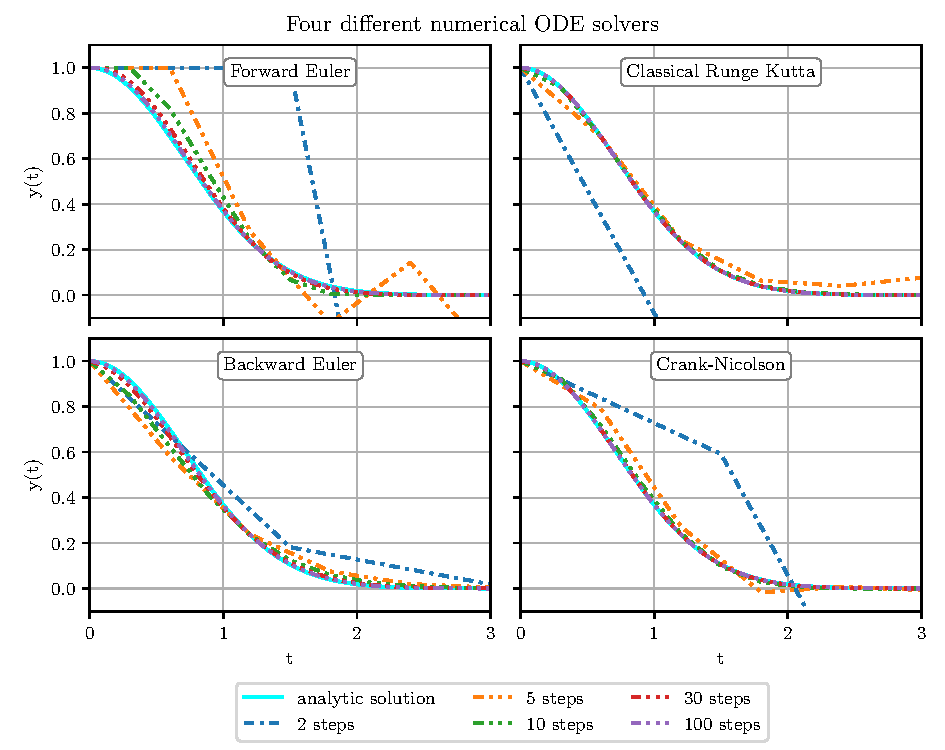
\includegraphics[width=17cm]{../Task_01/ODE_solvers.pdf}
    \caption{The approximations for the solution of the differential equation for each of the
    individual methods. It is nicely visible how an increase in integration steps leads to
    higher accuracy in the solutions.}
    \label{fig:ODE_solvers}
\end{figure*}

\subsection{Task 2}%
\label{sub:task_2}

For the second task a structure similarly to Task 1 was established. The script consists of
three functional functions that are needed for the Runge-Kutta-Fehlberg method namely
\verb+get_k()+, \verb+optimize()+ and \verb+rk45()+. Furthermore, a main function was written
to test the method using different tolerance factors \(\alpha\) ranging from \(10^{-1}\) to
\(10^{-6}\). The differential equation with its initial condition are given below:
\begin{eqnarray}
    \label{equ:init_cond_2}
    y(t=0) & = & 1 \\ \label{equ:ode_2}
    \frac{dy}{dt} & = & 0.1 y + \sin(t)
\end{eqnarray}

\subsubsection*{Initializing function call}%
\label{ssub:general_function_call}

To solve the differential equation, a general function call is invoked that initializes the
entire solving process. The function used for this is called \verb+rk45()+ and is a wrapper for
all more complex computations are then outsourced to the two helper functions \verb+optimize()+
and \verb+get_k()+. This wrapper takes the following arguments.
\begin{itemize}
    \item \verb+function+: The derivative \(\dot{y}(t)\) of the function \(y(t)\) that shall be
        determined.
    \item \verb+init_cond+: The initial condition of the differential equation.
    \item \verb+tolerance+: The Local Truncation Error tolerance factor \(\alpha\) that shall
        be used to work out the optimal time step.
    \item \verb+init_t_step:+: The initial time step guess.
    \item \verb+t_start+: Start time for the integration.
    \item \verb+t_end+: End time for the integration.
    \item \verb+logfile+: The name of the logfile to store intermediate results to.
\end{itemize}
The return value of this function is a four dimensional \verb+numpy.array+ that holds the time
\(t\) of the function value \(y(t)\), function value \(y(t)\), the length of the time step used
and the Local Truncation Error. Since the number of time steps is not fixed as the length of
said step is redetermined in each iteration, a python list ist used to store the results on the
fly and are only converted to a \verb+numpy.array+ when returned. As mentioned in Subsection
\ref{sub:classical_runge_kutta} the Runge-Kutta-Fehlberg method is defined by its Butcher
Tableau, see Table \ref{tab:rkf_butcher_tableau}. The Butcher Tableau is hardcoded in this
function as a multidimensional array. First three arrays, \verb+A+,~\verb+B+~and~\verb+C+,
corresponding to the three sections in any Butcher Tableau, see Table
\ref{tab:general_butcher_tableau}, are defined. These are then stacked into a single array so that the whole
table can be passed to the helper functions. The computations for the function values are done
in a while loop that checks if the current time is within the integration interval. Within this
loop the \verb+optimization()+ function is called.

\subsubsection*{Optimization}%
\label{ssub:optimization}

This is the module where the magic happens. The function arguments that are needed are listed
here.
\begin{itemize}
    \item \verb+function+: The derivative \(\dot{y}(t, y)\) of the function \(y(t)\) that is to
        be determined.
    \item \verb+time+: The current time of the time step.
    \item \verb+y_n+: Current function value \(y(t)\) from which the next function value
        \(y_{n+1}(t)\) is derived.
    \item \verb+delta_t+: The current time step length \(\Delta t\).
    \item \verb+tolerance+: The tolerance factor \(\alpha\) used for LTE\textsubscript{tol}.\\
        \(\mathrm{LTE}_\mathrm{tol} = \alpha y_n\)
    \item \verb+butcher_tableau+: A \verb+numpy.array+ containing the Butcher Tableau of the
        RK-method.
    \item \verb+logfile+: The file path or name of the logfile. All intermediate results are
        dumped into that file.
    \item \verb+rec_depth+: The number of times this function was called recursively.
\end{itemize}
This function has four return values, they are mentioned above. The first thing that happens in
this subroutine is the computation of the \(k_i\) coefficients according to Equation
\ref{equ:general_rk_method_2} using the Butcher Tableau. For this the helper function
\verb+get_k()+ is used, which takes \verb+function+, \verb+time+, \verb+y_n+, \verb+delta_t+
and \verb+butcher_tableau+ as arguments. Next the fourth and fifth order approximations are
computed, again using the Butcher Tableau, and the Local Truncation Error is determined. Now
the optimal time step length is estimated and compared to the one passed to the function in the
first place. If the initial time step is greater than the optimal time step, the optimization
is repeated with \(\Delta t_\mathrm{opt}\) as the initial time step. Otherwise \(\Delta t\) is
updated with \(\Delta t_\mathrm{opt}\), the time is advanced by \(\Delta t_\mathrm{opt}\) and
finally the results are returned with the fifth order estimate as \(y_{n+1}\).

\section{Results}%
\label{sec:results}

\subsection{Analytic solution}%
\label{sub:analytic_solution}

The analytic solution is quite easy to determine by using separation of variables. The full
derivation follows here.
\begin{eqnarray}
    \label{equ:analytic_solution}
    \frac{dy}{dt} & = & -2ty \\
    \frac{1}{y} dy & = & -2t dt \\
    \int \frac{1}{y} dy & = & -2 \int t dt \\ 
    \ln y & = & -2 t^2 + \tilde{c} \\
    y(t) & = & \exp\left(-2 t^2\right) c
\end{eqnarray}
With the initial condition \(y(t=0) = 1\) we determine the integration constant.
\begin{eqnarray}
    \label{equ:analytic_solution_2}
    y(0) = 1 & = & \exp\left(-2 * 0\right) c \\
    c & = & 1
\end{eqnarray}
Thus the complete solution is as follows.
\begin{equation}
    \label{eqn:analytic_solution_2}
    y(t) = \exp\left(-2 t^2\right)
\end{equation}

\subsection{Task 1}%
\label{sub:res_task_1}

As expected, the number of integration steps greatly influences the accuracy of the result. As
can be seen in Figure \ref{fig:ODE_solvers}, all methods perform badly with less than 30 steps.
With only two iterations, the computations greatly over or undershoots the analytical solution,
which is plotted as the solid line in all four cases.

\subsection{Task 2}%
\label{ssub:res_task_2}
\begin{figure}[htbp]
    \centering
    \captionsetup{width = 0.9 \linewidth}
    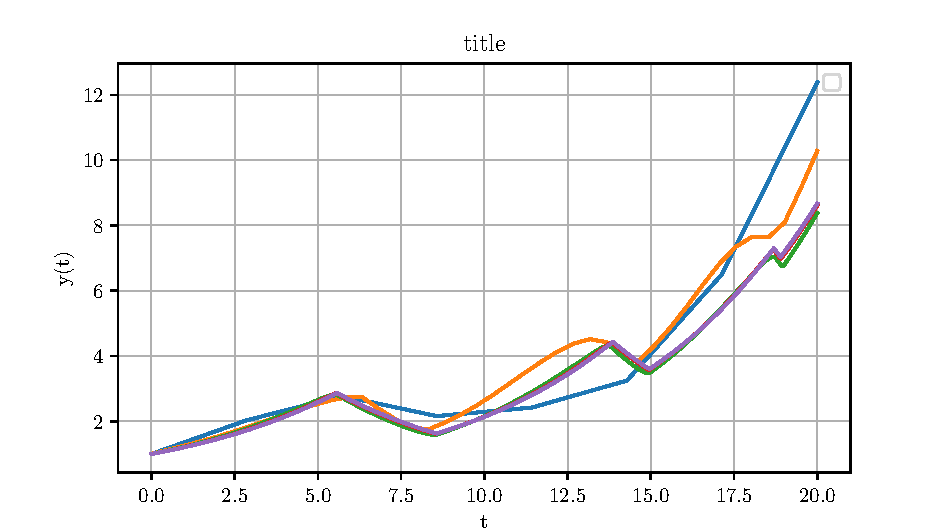
\includegraphics[width=\linewidth]{../Task_02/runge-kutta-fehlberg.pdf}
    \caption{The results of the RK45 method computed with different tolerance factors \(\alpha
    = [10^{-1} \dots 10^{-6}]\). The top plot shows the results for the differential equation.
    The middle depicts the time step length. Clearly visible are the variation in the length,
    especially with a LTE tolerance of \(10^{-4}y_n\), which is the red line close to the
    bottom. The bottom plot shows the number of integration steps needed for solution with
    specific tolerance.}
    \label{fig:res_rkf}
\end{figure}
Again, when taking a look at Figure \ref{fig:res_rkf}, the accuracy of
the approximation increases with smaller tolerances. Generally speaking, we start to get pretty
good results once the tolerance dips under \(10^{-4}y_n\). Also we can see in bottom plot, that
the number of iterations increases rapidly with a lower tolerance.

\end{document}
